\documentclass[conference,compsoc]{IEEEtran}

% *** CITATION PACKAGES ***
%
\ifCLASSOPTIONcompsoc
  % IEEE Computer Society needs nocompress option
  % requires cite.sty v4.0 or later (November 2003)
  \usepackage[nocompress]{cite}
\else
  % normal IEEE
  \usepackage{cite}
\fi
%\usepackage{graphicx}
%\usepackage{subcaption}
\usepackage{graphicx}
\graphicspath{ {images/} }
\usepackage{listings}
\usepackage[final]{pdfpages}
\usepackage{multicol}
\usepackage{dblfloatfix}
% correct bad hyphenation here
\hyphenation{op-tical net-works semi-conduc-tor}


\begin{document}
\begin{titlepage}
	\centering
	
\includegraphics[width=0.5\textwidth]{McGill_Logo}\par\vspace{1cm}
	{\scshape\LARGE McGill University \par}
	\vspace{1cm}
	{\scshape\Large ECSE 415 Project\par}
	\vspace{1.5cm}
	{\huge\bfseries Cat and Dog\par}
	\vspace{2cm}
	{\Large Jaeho Lee\par}
	{ 260633759\par}{			\par}	{		\par} {\Large Raymond So \par} {260640297 \par}{Team name: You thought it was an original team name, \\but it was me, DIO!}
	\vfill
	submitting to\par
	Prof.~James \textsc{Clark}

	\vfill

% Bottom of the page
	{\large \today\par}
\end{titlepage}
%
% paper title
% Titles are generally capitalized except for words such as a, an, and, as,
% at, but, by, for, in, nor, of, on, or, the, to and up, which are usually
% not capitalized unless they are the first or last word of the title.
% Linebreaks \\ can be used within to get better formatting as desired.
% Do not put math or special symbols in the title.
\title{ECSE 415 Project\\ Cat and Dog}
\author{\IEEEauthorblockN{Jaeho Lee \IEEEauthorrefmark{1} and Raymond So \IEEEauthorrefmark{2}}
\IEEEauthorblockA{Department of Electrical Engineering, McGill University\\
\IEEEauthorrefmark{1}jaeho.lee2@mail.mcgill.ca, \IEEEauthorrefmark{2}raymond.su@mail.mcgill.ca}}

\maketitle



\IEEEpeerreviewmaketitle

\section{Introduction}
% no \IEEEPARstart
Most research for object classification was more focused on classifying images that are completely different (e.g. horses and boats). In this project, we classify whether the image contains a picture of dog or cat. We were provided a training set of 5906 images from [1]. We trained animal body detection using Haar feature-based classifiers with 1500 images of cats and 1500 images of dogs. Once these classifiers were trained, they were used to detect animal bodies in the training set, and the local binary pattern (LBP) histograms of the portion of the image containing the animal were computed. These histograms provided the features used to train a support vector machine (SVM) classifier model that can determine whether there is a cat or a dog in a photo. These steps were taken a second time to create an SVM classifier that detects and classifies the animals based on their faces rather than their entire bodies.

\section{Problem Representation}
The goal of this project is to devise a machine learning algorithm to analyse images and classify them based on whether there is a cat or a dog in the image. The datasets for training and testing, which together consist of 7384 images, were provided at [7]. The ratio of dog images to cat images in the given training dataset was 2:1, so if all of them were used in training, there may be a significant bias towards categorizing images as dogs. In order to fix this data inequality, we used external datasets from [8] which includes 4004 cat face images, and 2271 cat ear images. \\

To tackle this problem, we built a face detector and a body detector in order to limit features to be classified. Face detection is run first because it is easier and can more accurately detect animal faces than the body detector can detect animal bodies. This is because face data is more consistent than body data, which makes sense considering that the animals can be in any number of different positions. In addition, some photos might not include the animal's entire body, whereas the face is almost always shown in the image. In [5], using classification based on face detection performed better than using body detection. We used Haar feature-based detection from [2] for both face detection and body detection\\

We used LBP histograms from [4] as the features to be used for classification, because LBP is fast and simple to compute, and it is proven to perform well in classification based on facial features [4]. After extracting the histogram data, Linear Support Vector Machine (LSVM) training was used to generate a model that was used to classify whether the image includes a cat or a dog.
\begin{figure*}
	\begin{multicols}{4}
    		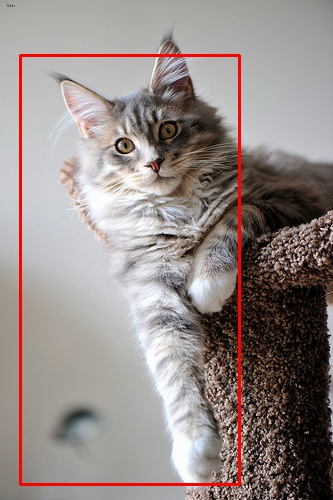
\includegraphics[height=1.35\linewidth]{naisubodi2.jpg}\par 
    		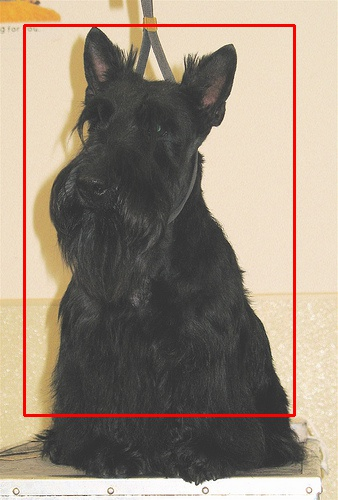
\includegraphics[height=1.35\linewidth]{good3.jpg}\par 
    		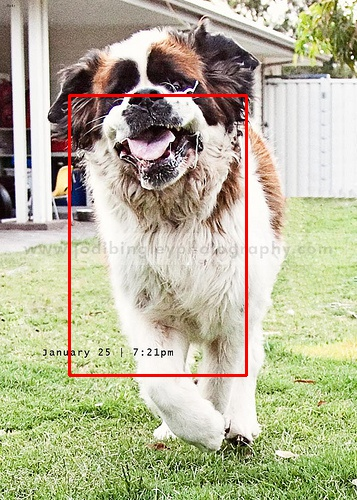
\includegraphics[height=1.35\linewidth]{terrible1.jpg}\par
    		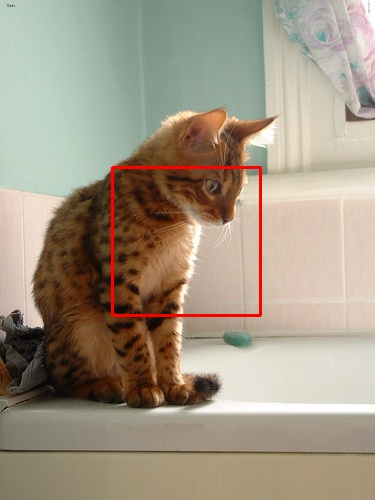
\includegraphics[height=1.35\linewidth]{terrible5.jpg}\par
	\end{multicols}
	\caption{Body detection result (left : succeed, right : failed)}
\end{figure*}
\begin{figure*}
	\begin{multicols}{4}
    		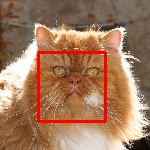
\includegraphics[height=1.35\linewidth]{goodFace2.jpg}\par 
    		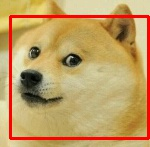
\includegraphics[height=1.35\linewidth]{dogeFace.jpg}\par 
    		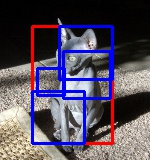
\includegraphics[height=1.35\linewidth]{smolrect.jpg}\par
    		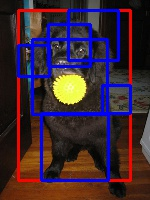
\includegraphics[height=1.35\linewidth]{smolrect2.jpg}\par
	\end{multicols}
	\caption{Face detection result (left : succeed, right : failed)}
\end{figure*}
\section{Algorithm selection and implementation}
We used Haar a feature-based cascade classifier from [2] to identify the relevant portion of the image  because it performs quickly and accurately [2]. We used the pre-built OpenCV annotation program to manually select face and body regions for each image used. For body detection training, we used 3000 images from the [7] dataset. For face detection training, we used 8000 images from [7] and [8] dataset. The annotation program generated a text file containing all the selected image regions, and this information was then stored in a vector file using the built-in OpenCV createsamples program. After creating vector file, we used it, along with roughly 20000 negative images from [6], in OpenCV's built-in traincascade program to train the cascade classifier create to create an xml file with the classifier data. We used a 14 stage classifier for face detection and a 17 stage classifier for body detection. Before detecting faces using test images, we used a Gaussian filter to simplify features, which increased detecting performance. Despite this, there were still cases where the face and body detections failed. Figure 1 shows successful and failed face detection examples, and figure 2 shows successful and failed body detection examples.\\

After object detection, we used LBP from [4] and obtained the histogram of the face or body part, which was the feature used for SVM classification training. If the face detection program failed to detect face, the body detection would activate instead. We trained 3804 images for LBP from [7]. The LBP of the entire detected region was used rather than dividing the region into smaller cells because the detected dog or cat face often ends up being very small, therefore it would not be worth it to use multiple cell LBP.\\

LinearSVC from sklearn library [9] was used to create a linear separation between dog and cat features.


\section{Testing}
This project is separated into two different sections, object detection and classification.  This section describes how they were tested and the result of the project.
\subsection{Object Detection}
For both face and body detection, we trained the cascade classifiers with different numbers of stages, different distributions of face types, and different section of faces. With 4000 face samples, the cat face detector performed best with 14~16 stages. Above 16 stages, the classifier would not detect anything frequently because the classifier was overtrained. Below 14 stages, the detector detects false positives and adds unnecessary parts which defeats the purpose of face detection, even with the optimized stages, as shown in Figure 2. The images on the right do show properly detected faces, however they also include other unnecessary parts which ruined the face detection. Considering the test image set animal heads shown in various different angles, we distributed cat face photo before training. Out of 4000 cat face photos, we used 2500 front-facing open eye faces, 800 front-facing closed eye faces, and 700 side view of the cat face which improved the performance in general. We also trained an additional cascade classifier consisting of cat ears only. We used 2100 cat ear photos and ran the detection with cat face classifier. However this did not improve the performance therefore we discarded it.\\

In case of the body detector, it detects the entire or major parts of animal. Even in the failed cases, the detector succeeds in detecting the body of animal but did not include the entire body. However since part of animal is included we still could use the SVM classifier to deermine whether the animal is a cat or a dog. However, the classification performance would drop because using entire body gives numerous characteristics which overwhelms LBP histogram classification [5].
\subsection{Classification}
After classification, we obtained 66.6\% of accuracy which was below our expectation. The labels in the csv file consist  mostly of 1s which indicates the SVM is biased towards dog. We suspect several different reasons which are briefly discussed in section 5.

\section{Discussion}
The positive aspects of our methodology are that face detection has been proven to be a better way to classify images than body detection, and the face detection did work in most cases. The implementation of the classification training is where this method fell short. \\

There could be multiple reasons why the classification did not perform as well as we expected. We concluded that this was because the SVM training is biased to dog side, or because our face detection did not work well enough. One possible improvement that could be made to the face detector to implement it by detecting smaller regions of the face, such as the eyes and nose, and then combine them to obtain the face region of the image. Another possible improvement would be to split the face region into smaller cells when performing LBP, which would provide a much more accurate descriptor for the face than the single global descriptor currently being used. Another possible improvement would be the use of clustering to extract the animal portion of the image from the background before classifying it to reduce the noise introduced by the background, but this is very difficult to do automatically. For the classifier, we could also use Adaboost to expand the region allocated to the cat class in the feature space, which would increase number of cat classifications. If classifying using either the entire body or face, we could use Central Neural Network (CNN) technique for both the classifier and the detector [3]. CNN requires more computing power and more data for training, but it would solve problems caused by the animals being in different positions, or only a certain part of the animal is shown. Histogram of Ordered Gradient (HoG) could be an alternative solution for the detector which uses multiple small feature windows and merges them to make one large detection window [10].

%\begin{thebibliography}{1}

%\bibitem{IEEEhowto:kopka}
%T~.Ahonen, et al., \emph{Face Description with Local Binary Patterns: Application to Face Recognition}, 7th~ed. New York, NY, United States: Oxford University Press, 2014.

%\end{thebibliography}

%\onecolumn

\begin{thebibliography}{9}

%Conference
\bibitem{lamport94}
	O. M. Parkhi et al.,
	"Cats and Dogs," in 
	\emph{IEEE Conference on Computer Vision and Pattern Recognition} , 2012.

%Conference
\bibitem{lamport94}
	P. Viola and M. Jones,
	"Rapid Object Detection using a Boosted Cascade of Simple Features, " in
	\emph{Conference on Computer Vision and Pattern Recognition}, 2001.
		
%Conference
\bibitem{lamport94}
	Y. Taigman et al.,
	"DeepFace: Closing the Gap to Human-Level Performance in Face Verification," in
	\emph{2014 IEEE Conference on Computer Vision and Pattern Recognition,}  Columbus, OH, 2014, pp. 1701-1708.

%Journal
\bibitem{lamport94}
  T Ahonen et al.,
  "Face Description with Local Binary Patterns: Application to Face Recognition,"
  \emph{IEEE Trans. Pattern Anal. Mach. Intell},, vol. 28, no.12, pp.2037 - 2041, dec. 2006.
  
  
%Technical Report
\bibitem{lamport94}
	C. Wang and L. Jiang,
	"Recognizing Cats and Dogs with Shape and Appearance based Models," McGill Univerisy, Montreal, QC, 2013.

%Tecnhical Report
\bibitem{lamport94}
	G. Griffin et al.,
	"Caltech-256 Object Caegory Dataset," California Institute of Technology, Pasadena, CA, 2007.

%Website
\bibitem{lamport94}
	G. Corcoran. (2017, March 23). ECSE 415 Classification [Online]. Available: https://inclass.kaggle.com/c/ecse415-classification/data

%Website
\bibitem{lamport94}
	T. M. (2011, Jan 17). CatDataCollection [Online]. Available: https://sites.google.com/site/catdatacollection/data
	
%Website
\bibitem{lamport94}
	A. Mueller. (2016, Aug 3). sklearn.svmLinearSVC [Online]. Available: http://scikit-learn.org/stable/modules/generated/sklearn.svm.LinearSVC.html

%
\bibitem{lamport94}
	P. F. Felzenszwalb et al., 
	"Object Detection with Discriminatively Trained Part-Based Models," in
	\emph{IEEE Transactions on Pattern Analysis and Machine Intelligence,} vol. 32, no. 9, pp. 1627-1645, Sept. 2010.
	 

\end{thebibliography}

\end{document}


